\chapter{Modelling The Energy Usage And Carbon Emissions Of Ethereum}
\label{Modelling}

% ____________________________________________________________________________
\section{Chapter Summary}


% ____________________________________________________________________________

%  MODEL AAAAAAAAAAAAAAAAAAAAAAAAAAAAAAAAAAAAAAAAAA
\subsection{Model A}
From the research,it seems like power usage is usually not the limiting factor but rather the storage space needed to run validators.

The recommended hardware for a validator one is shown in table \_\_ of the appendix as well as in the table below. \_\_

So according to this hardware recommendation, we could estimate the power usage depending on statistics provided by manufacturers. Let's assume the same configuration of hardware as in the \cite{CryptoCarbonRatingsInstitute2022TheNetwork} (They don't mention type of power supply and mainboard).  According to data from the manufacturers, the power consumption for this configuration comes out to the following: 

\begin{itemize}
    \item Processor TDP - 105W
    
    \item An SSD uses 5W while Active
    
    \item Every 8GB of memory uses 3W, so 16GB of memory will use 6W
    
    \item For a solo validator set-up (non-specialised hardware), miscellaneous components are likely to use another 30W
    
    \item As 92\% efficiency is common, the machine will likely peak at 178W of AC power drawn from the wall
    
    \item The machine will run at idle power consumption 50-90\% of time, so on average it would use around 50-100W
    
\end{itemize}

% _____________________________________________________________________________
%  MODEL BBBBBBBBBBBBBBBBBBBBBBBBBBBBBBBBBBBB
\section{Model B: Parametric Modelling with Prior Domain Knowledge}

% \textbf{Light Nodes}
% Light nodes require much less computational power to run compared to a full node, yet, they still work in a trust-minimised way. This is due to their cryptographically proven way of using block headers of the blockchain to verify the information they are receiving from a full 
% node themselves. 

% Light clients send out a lot of requests, a lot more than full nodes. For example, they might need to check the balance of certain accounts to verify the information they are receiving cryptographically. This large number of simple requests ends up requiring more network bandwidth than full nodes \cite{WhatTechnologies}. We also know that light clients are designed to be run on minimal devices such as mobile and IoT devices. The amount of computational and storage resources required by a light node is orders of magnitude lower than a full node. It requires only about 100MB of storage \cite{WhatTechnologies}. This fact can be used to model this. These devices also sync with the latest blocks using checkpoints in seconds instead of hours like a full node.

% _____________________---stage 1
\textbf{The CRRI Equation Adapted}

This section introduces the CCRI equation for the 'weighted  electricity  consumption  of  an  average  node for each combination of one consensus and one execution client'\cite{CryptoCarbonRatingsInstitute2022TheNetwork} with symbols adapted for this paper. Power and electricity are synonymous below.

A Consensus Layer Client's power usage is denoted by subscript:
\begin{equation*}
    \boldsymbol{\mathrm{P}_{CL}}
\end{equation*}

An Execution Layer Client's power usage is denoted by subscript:
\begin{equation*}
    \boldsymbol{\mathrm{P}_{EL}}
\end{equation*}
 
 An Idle client's power usage is denoted by: \begin{equation*}
    \boldsymbol{\mathrm{P}_{ID}}
\end{equation*} 

Mean Electricity usage for each of the 3 client types are denoted by the following respectively: 
\begin{equation*}
  \boldsymbol{\mathrm{{\overline{P}}_{CL}}}\quad      \boldsymbol{\mathrm{{\overline{P}}_{EL}}}\quad  \boldsymbol{\mathrm{{\overline{P}}_{ID}}}   
\end{equation*}

The number of machines ran with different combinations of consensus and execution layer clients is denoted by:
\begin{equation*}
    \boldsymbol{n}
\end{equation*}

The known share of the network that uses a specific combination of Consensus and Execution layer client is denoted by:
\begin{equation*}
    \boldsymbol{\phi}_{EL,CL} \text{ where } {i} \text{ represents a specific CL and EL client combination.}
\end{equation*}

The total share of the network occupied by ${n}$ tested combinations of consensus and execution layer clients is denoted by:
\begin{equation*}
    \boldsymbol{{\pi} = \displaystyle\sum\limits_{i=1}^{n}{\phi_{EL,CL}}}
\end{equation*}

The final equation: 

\begin{equation}
\boldsymbol{\frac{\displaystyle\sum\limits_{i=1}^{n}{ \left({\left(\mathrm{\overline{P}}_{ID} + \mathrm{\overline{P}}_{CL} + \mathrm{\overline{P}}_{EL}\right)} * {\phi_{EL,CL}} \right)}}
 {\pi}}\label{eqn:CCRI}
\end{equation}



% ____________________stage 1
\textbf{Stage 1: Adding the Synchronisation Energy} 

 The equation \ref{eqn:CCRI} ignores the energy expended during the bootstrapping stage of running a node - the synchronisation process. Geth is the most dominant (\tref{Table:tabsubex}) and long-standing Ethereum EL client. Geth's snap sync mode is the most commonly used sync mode as it strikes a great balance between independent verification and sync speed.
% DIAGRAM FOR SNAP SYNC
 All types of syncing modes are very energy-intensive and snap-sync is no exception. It works by downloading the headers of chunks of blocks at a time and verifies these. In parallel to this it starts downloading the state-trie for each block and cryptographically verifying this by regenerating it locally. These computationally intensive processes utilise the CPU to its maximum capacity.

  % keeping Intel i5-1135G7 in mind
The model for calculating the energy consumption of a CPU introduced by this paper \cite{SaingreUnderstandingContracts} is shown below:

\begin{equation*}
    \boldsymbol{\mathrm{P}_{Total} = \mathrm{P}_{idle} + \left({\mathrm{P}_{max} - \mathrm{P}_{idle}}\right) * \mathrm{U}}
\end{equation*}

Where $\boldsymbol{\mathrm{P}_{Total}}$ is the total energy consumption of the CPU, $\boldsymbol{\mathrm{P}_{idle}}$ and $\boldsymbol{\mathrm{P}_{max}}$ denote the power consumption of the CPU in an idle state and under maximum load. $\boldsymbol{\mathrm{U}}$ denotes the percentage of CPU usage under load.

In our case, we want to capture only the energy consumption of the syncing process. For the sake of simplicity, we will assume the $\boldsymbol{\mathrm{U}}$ to be 100\%, or $\boldsymbol{1}$. This negates the need for $\boldsymbol{\mathrm{P}_{idle}}$ to be included in the equation:

\begin{equation*}
    \boldsymbol{\mathrm{P}_{Total} = {\mathrm{P}_{max}}}
\end{equation*}

This paper \cite{Schuchart2016TheScale} shows that the processor cannot continuously operate at maximum capacity for computationally intense applications. To cope, it reduces it's frequency, maintaining operations within the thermal power limitation, the TDP. Hence the TDP can be used as an accurate measurement of the energy consumption of a CPU under a high sustained load. We can infer: \label{TDPReasoning}

\begin{equation*}
    \boldsymbol{\mathrm{P}_{max} = {\mathrm{P}_{TDP}}}
\end{equation*}

Where the TDP (Thermal Design Power) of the CPU being used by the node is denoted by $\boldsymbol{\mathrm{P}_{TDP}}$, measured in Watts. This can easily be found on the CPU manufacturer's website.

While the CPU is being utilised at maximum capacity, the node also begins storing this information locally to assemble a local copy of the chain in parallel. This storage process requires speeds that hard drives cannot keep up with. This is reinforced by the recommended specs shown in the \tref{Table:RecommendedHardware} which requires an Solid State Drive with DRAM. These are much faster than traditional hard drives and expend more energy as a consequence. 

 The average energy estimation of an SSD actively in use, in Watts, is denoted by:
 \begin{equation*}
    \boldsymbol{\mathrm{P}_{SSD}} 
\end{equation*}

Often, it takes days to complete a full sync. The time it takes to complete the synchronisation process, in hours, is denoted by:
\begin{equation*}
    \boldsymbol{\mathrm{T}_{SNC}}
\end{equation*}

Thus the total power expended during the synchronisation process $\boldsymbol{\mathrm{P}_{SNC}}$ can be represented as:
\begin{equation}
    \boldsymbol{\mathrm{P}_{SNC} = \mathrm{T}_{SNC} * \left({\mathrm{P}_{TDP}} + \mathrm{P}_{SSD}\right)} \label{eqn:Sync}
\end{equation}

As this is a bootstrapping process, integrating equation \ref{eqn:Sync} into the CCRI equation \ref{eqn:CCRI} results in the following:

\begin{equation*}
    \boldsymbol{\mathrm{P}_{SNC} +  {\frac{\displaystyle\sum\limits_{i=1}^{n}{ \left({\left(\mathrm{\overline{P}}_{ID} + \mathrm{\overline{P}}_{CL} + \mathrm{\overline{P}}_{EL}\right)} * {\phi_{EL,CL}} \right)}}
 {\pi}} } 
\end{equation*}

Which simplifies to:

\begin{equation}
     \boldsymbol{\left({\mathrm{T}_{SNC} * \left({\mathrm{P}_{TDP}} + \mathrm{P}_{SSD}\right)}\right) +  {\frac{\displaystyle\sum\limits_{i=1}^{n}{ \left({\left(\mathrm{\overline{P}}_{ID} + \mathrm{\overline{P}}_{CL} + \mathrm{\overline{P}}_{EL}\right)} * {\phi_{EL,CL}} \right)}}
{\pi}} } \label{eqn:CCRISync}
\end{equation}

\textbf{ Stage 2: Running multiple validators per client}
As the data suggests, there are roughly always 11-15000 nodes online at any given moment \cite{NodewatchAnalytics}, meanwhile, there are 561,472 validator instances running \cite{EthereumEthereum.orgc}, as of 28 Mar 2023. It is known that most solo-stakers run 1-1000 validator instances per physical node. With more specialised hardware, 2500-7000 validators can be run on a single node \cite{Kaushal2022ValidatingConference}. 

This can only be possible if the cost of adding each additional validator puts negligible strain on the physical node. The graph in \fref{Figure:validatorIncrease} \cite{Sutton2022ExploringSymphonious} plots the CPU usage (green line, left axis) and rate of gossip messages per second (blue line, left axis) against a gradually increasing number of validators (yellow line, right axis) running on a single machine.

\begin{figure}[htb!]
    \centering
    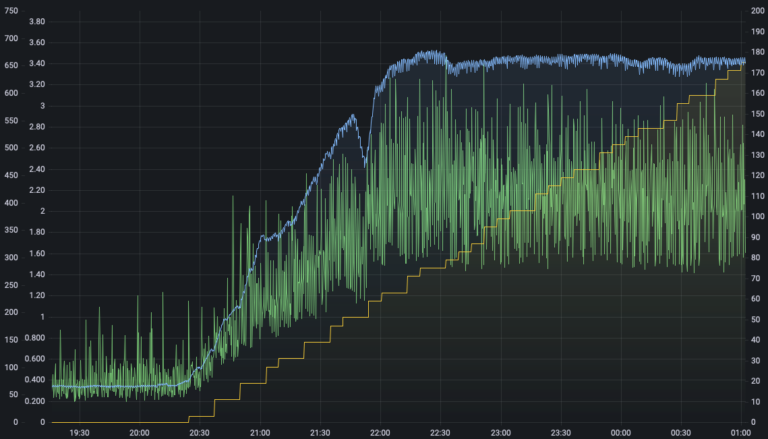
\includegraphics[width=15cm,center]{Figures/cpuValidatorsGossip.png}
    \caption{Graph showing the effect on CPU usage (green line, scale up to 3.80 in GHz) and gossip messages per second (blue line, scale up to 750 messages/sec ), as the number of validators running on one node increases (yellow line, scale up to 200 clients). \cite{Sutton2022ExploringSymphonious}}
    \label{Figure:validatorIncrease}
\end{figure}

An expected linear correlation can be seen between the increasing number of validators and CPU usage, but only up to 60 validators. However, after the 60-70 validator range, the CPU usage and the gossip messages per second level off and seem unaffected by the steadily increasing validators. Other sources that support  this finding - \cite{Roy2022StakingExchange} and \cite{2021HardwareEthstaker}.

Storage space was falsely expected to be a limiting factor as running a single validator takes up almost 2TB of storage. However, after the first validator already has a local copy of the blockchain synced, adding more validators only requires storing a few extra validator keys.

This finding can be explained by understanding Sharding and attestations(section \ref{Sharding}). In each epoch (an epoch has 32 slots), 32 randomly selected block proposers propose one block per slot. The remaining validators are not only assigned 1/32 slots that they need to attest the new block for (vote on its validity) but also to possibly one of 64 voting committees. Unaggregated votes from these committees are aggregated and pushed out on specific gossip channels by certain validators assigned to do so. 

Nodes that are not running validators will only subscribe to the gossip topics that push out aggregated votes. But with each validator that you run, they will first need to subscribe to gossip channels with aggregated attestations but occasionally also to gossip topics with unaggregated attestations if they're selected to aggregate the votes for that slot. Hence, up to 64 validators, validators are subscribing and processing more and more gossip messages but past this, there are no new gossip topics to subscribe to and the CPU usage and gossip messages per second level off, as shown in \fref{Figure:validatorIncrease}.

We tried to replicate this behaviour using logarithmic functions and exponential decay functions. Through extended experimentation and applying prior knowledge, we found that the exponential decay function (increasing form), equat{eqn: ExpDecayGeneral} ref{eqn: ExpDecayGeneral}, most accurately matches the characteristics we are looking for because it increases at a slower rate at the beginning and then levels off as more validator clients are added to the node. This is consistent with \ref{Figure:validatorIncrease} that grows almost linearly until 64 validators, after which it levels off. The general equation is:

\begin{equation}
    \label{eqn: ExpDecayGeneral}
    \boldsymbol{\mathrm{E(\mathrm{x})} = \mathrm{A} (1-\mathrm{e}^{-\mathrm{k}(\mathrm{x})}) + \mathrm{C}}
\end{equation}

The lower limit or Y-intercept, $\boldsymbol{\mathrm{C}}$, can be set to the energy measurement obtained for running a single validator client on a specific hardware configuration of a node. As seen in \ref{Figure:validatorIncrease}, the CPU approaches its maximum capacity as the number of validators approaches 64, after which it levels off, but the SSD is not working to its maximum capacity. Hence, the asymptotic upper limit of the graph $\boldsymbol{\mathrm{A}}$, can be set to $\boldsymbol{\mathrm{P}_{TDP}}$ assumed to be due to the aforementioned reasoning (section \ref{TDPReasoning}). The equation already has its lower limit set to running a single validator, and this equation will only be employed for cases where there are multiple validator clients being run on a single node. Thus, $\boldsymbol{\mathrm{x}}$ denotes the number of additional validator clients run on a node and can only take values from the set of all positive integers.  $\boldsymbol{\mathrm{k}}$, the growth rate constant determines how quickly the energy consumption increases as the validators increase and can be calculated for each node on a case-by-case basis. However, to simplify the equation, we can remove the $\boldsymbol{ + \mathrm{C}}$ as it simply acts as a transition upwards to the graph output by this equation. This modification leaves an equation that outputs the extra electricity consumed by $\boldsymbol{\mathrm{x}}$ additional validators:

\begin{equation}
    \label{eqn:ExpDecay}
    \boldsymbol{\mathrm{E(\mathrm{x})} = \left(\mathrm{P}_{TDP} - \mathrm{C} )\right(1-\mathrm{e}^{-\mathrm{k}(\mathrm{x})}) \qquad \forall x \in \mathbb{Z}^+}
\end{equation}


\begin{figure}[htb!]
    \centering
    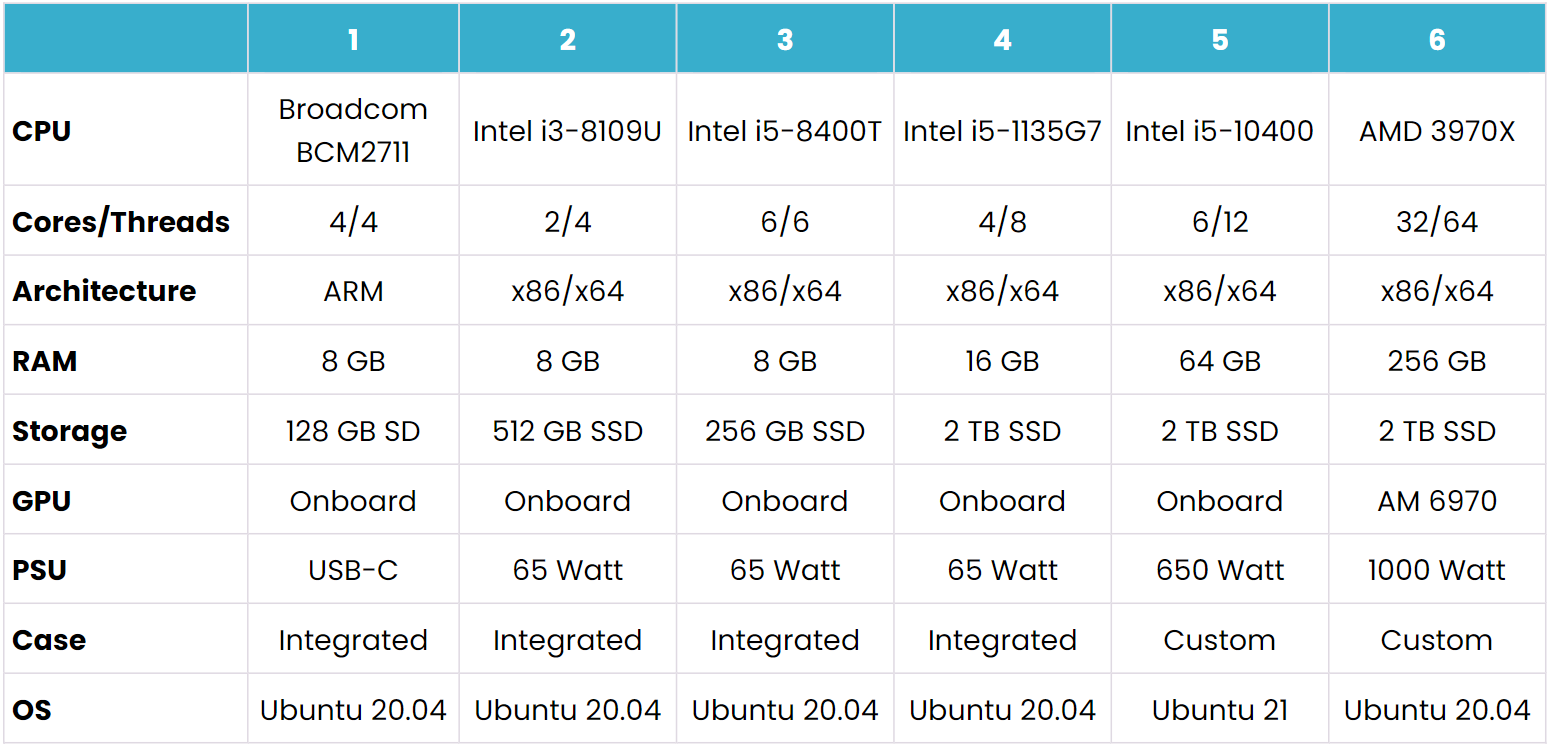
\includegraphics[width=15cm,center]{Figures/CCRIhardwareConfig.png}
    \caption{Table showing hardware configurations of low-tier, mid-tier and high-tier nodes relative to the hardware recommended to run a validator node shown in table \ref{Table:RecommendedHardware}. Source: CCRI report \cite{CryptoCarbonRatingsInstitute2022TheNetwork}, table 6.}
    \label{Figure:CCRIhardwareConfig}
\end{figure}

Here is an example calculation to determine constant $\boldsymbol{\mathrm{k}}$ for an average node, configuration 6, shown in figure \ref{Figure:CCRIhardwareConfig}. 

$\boldsymbol{\mathrm{C}} = \boldsymbol{\mathrm{150.20}} $ Watts, assuming the node runs the most common CL and EL client combination, Prysm and Geth. Mean values are taken from  \cite{CryptoCarbonRatingsInstitute2022TheNetwork}.

$\boldsymbol{\mathrm{A}} = $ TDP rating for AMD 3970X, $\boldsymbol{\mathrm{280}} $ Watts \cite{AMDDatabase} subtracted by the $\boldsymbol{\mathrm{C}}$ value which results in $\boldsymbol{\mathrm{129.80}}$ W.

We can set $\boldsymbol{\mathrm{x}} $ can be set to $\boldsymbol{\mathrm{63}} $, as the graph starts at 1 validator running already, totalling 64 validators. We assume that the CPU is operating at just 10\% below its maximum capacity (TDP rating) at the 64$^\mathrm{{th}}$ total validator and equate the left side of the equation to $\boldsymbol{\mathrm{0.9 * TDP}} = 252$ W. This needs to be subtracted by $\boldsymbol{\mathrm{C}}$ to account for translating the graph upwards earlier, resulting in $\boldsymbol{\mathrm{252-150.20 = 101.8}}$W. 

\begin{equation*}
    \boldsymbol{\mathrm{129.8} * (1-\mathrm{e}^{-\mathrm{k}(\mathrm{63})}) = \mathrm{101.80}}
\end{equation*}

Which solves to:
\begin{equation*}
    \boldsymbol{\mathrm{k} = \mathrm{{2.435} * {10}^{-2}}}
\end{equation*}

\begin{figure}[htb!]
    \centering
    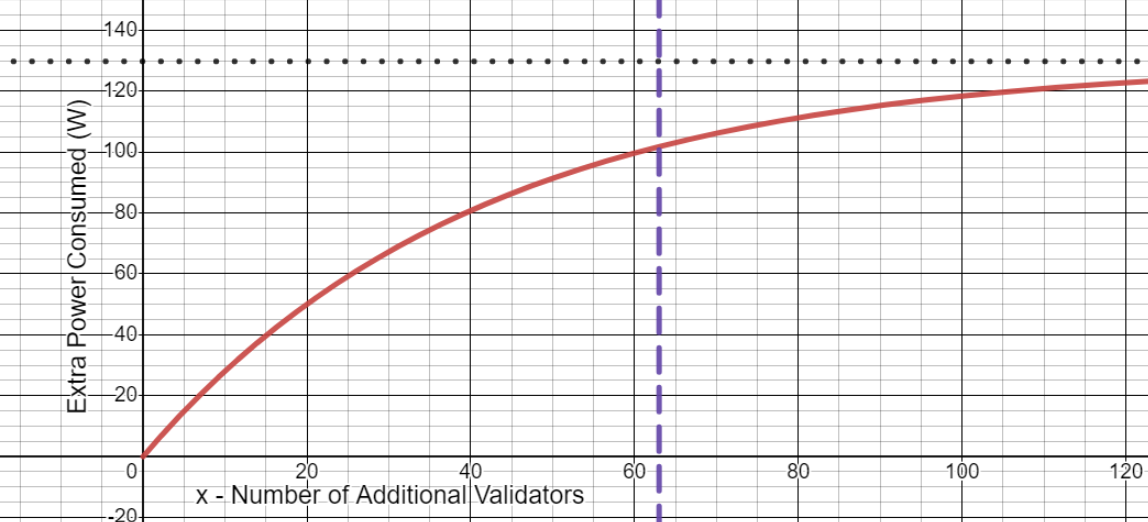
\includegraphics[ width=14cm,center]{Figures/AsymptoteMultipleValidators.png}
    \caption{A plot of equation \ref{eqn:ExpDecay} showing its asymptotic behavior. The asymptote at $\boldsymbol{\mathrm{A = 129.80}}$W is highlighted y the horizontal dotted black line. A dashed vertical purple line also highlights the value of the curve to be $\boldsymbol{\mathrm{101.8}}$W at $\boldsymbol{\mathrm{x = 63}}$}
    \label{Figure:MultipleValidators}
\end{figure}

Equation \ref{eqn:ExpDecay} is case specific and can be applied independently to estimate the electricity usage of a node with a specific combination of EL and CL clients as well as a specific hardware combination. To integrate this equation into the one proposed earlier, equation \ref{eqn:CCRISync}, it will need to be generalised, keeping all combinations of hardware and clients in mind.









% -------------------------------------------------------------------------------
\textbf{Assumptions:}

\begin{itemize}
    \item The TDP + SSD power usage can be used as an upper limit for the electricity consumption of any hardware set-up
    \item That growth for more than one validator can be modelled by an exponential decay (increasing form)
    \item This exponential growth has an upper limit of TDP + SSD power usage and using the single validator energy consumption as the lower limit
    \item Equation from CCRI gives an accurate estimation and is a good base for my equation
    \item The EL and CL layer clients are not changed; just additional Validator clients are run on the same set up
    \item 10\% lower then the TDP power should be reached by the time the 64$^\mathrm{{th}}$ validator is run.
\end{itemize}














% ___________________________________________________________________MODELS DONE< NOW 

% MODEL BBBBBBBBBBBBBBBBBBBBBBBBBBBBBBBBBBBBBB
\section{Model B Results}

\textbf{Data Gathering}
The recommended hardware configuration for a Geth client is shown in \tref{Table:RecommendedHardware}.

\begin{table}[h]
\centering
\begin{tabular}{|l|l|}
\hline
Solo Validator Nodes        & \begin{tabular}[c]{@{}l@{}}Quad Core Processor, \\ 2TB SSD , 16GB memory\end{tabular}                            \\ \hline
Archive Nodes               & \begin{tabular}[c]{@{}l@{}}Quad Core or Dual Core Hyperthreaded \\ Processor, 12TB SSD, 16GB memory\end{tabular} \\ \hline
Minimum for Validator nodes & \begin{tabular}[c]{@{}l@{}}Dual Core Hyperthreaded, \\ 1TB SSD, 4GB memory\end{tabular}                          \\ \hline
\end{tabular}
\caption{Recommended hardware configurations for running various nodes by Geth \cite{2022DeveloperGo-ethereum}}
\label{Table:RecommendedHardware}
\end{table}

A combination of hardware that closely matches the recommendation by Geth developers must be chosen. The following specification was chosen:
Intel i5-1135G7

config 5 
$65(1-e^(-63k))  + 37.61= 58.5$


Because it is a recent CPU, made to be in laptops. This is aligned with the aim of running PoS Ethereum nodes on commodity hardware. It is also a configuration with actual data in the report by \cite{CryptoCarbonRatingsInstitute2022TheNetwork} and hence will draw fair comparisons when the models are compared.



% ____________________________________________________________________________
\subsection{Ethereum's Total Network Energy Consumption}

% ____________________________________________________________________________
\subsection {Modelling Energy Consumption Per Transaction}

% ____________________________________________________________________________
\subsection{Assumptions}

\begin{itemize}
    \item They have taken the syncing on nodes into account into their model whereas for general modelling, it would be  abetter estimate to ignore this initial set up energy and get an avergae form then on. That is what this paper has done, taking averages of the Raspberry Pi rather than including the syncing energy.
    \item ding ding
\end{itemize}


% _____________________________________________________________________________
\section{ Data-Driven Model}
\subsection{Data Gathering}






% ______________________________________________________________________
\section {Modelling Ethereum's Carbon Emissions}
\url{https://ethernodes.org/countries}

\paragraph{ Simple Linear Regression Model}
A simple logical model for estimating the energy consumption of Ethereum 2.0's energy consumption logically would be using simple regression. y = mx + c, and if we wanted to say that energy is dependent on transactions, then we can say y is the energy per node, m is the slope we need to find, x is the number of transactions/sec, c is the base energy an idle node requires. Then we multiply this whole thing by the number of validators on the network to get the overall network energy consumption.

% ____________________________________________________________________________
\section{Discussion and Evaluation Of Models}
% ____________________________________________________________________________
\subsection{Results}
% ____________________________________________________________________________
\subsection{Interpretation}


% ____________________________________________________________________________
\subsection{Validation and Evaluation}


\tref{Table:tabsubex} shows updates values recorded by CCRI in their report \cite{CryptoCarbonRatingsInstitute2022TheNetwork} for model \_\_\_\_. %ADD HEREE_________

\begin{table}[!htb]
    \centering

  \subcaptionbox{\textbf{Execution Clients} \cite{Sigp/blockprint:Metrics}}{
      \begin{tabular}{|l|c|}
            \hline
             Geth & 69.22 \% \\
            \hline
             Nethermind & 14.16 \%  \\
            \hline 
             Erigon & 10.65 \% \\
            \hline
             Besu & 5.78 \% \\
            \hline
             OpenEthereum & 0.00 \% \\
            \hline
             Other & 0.20 \% \\
            \hline
  \end{tabular}
    \label{Table:tabsubex:left}
  }
  \subcaptionbox{\textbf{Consensus Clients}  \cite{ClientsExplorer}}{
        \begin{tabular}{|l|c|}
                    \hline
             Prysm & 65.15 \%  \\
            \hline
             Lighthouse & 29.30 \% \\
            \hline 
             Teku & 10.65 \% \\
            \hline
             Nimbus & 0.91 \% \\
            \hline
             Lodestar & 0.0 \% \\
            \hline
             Other & 0.0 \%  \\
            \hline
            
  \end{tabular}
    \label{Table:tabsubex:right}
  }
    \caption{An updated table of client diversity within Ethereum Mainnet network, data recorded on 27-Mar 23. Updates the table from report \cite{CryptoCarbonRatingsInstitute2022TheNetwork} }
  \label{Table:tabsubex}
\end{table}

Note that the OpenEthereum Execution client has been deprecated and is no longer being maintained. Thus, it is no longer included in the table.

% ____________________________________________________________________________
\subsection{Discussion}
*So I did it this way, could've been done another way. My method could've affected the results
* self-reflection -> smaller factors not considered, maybe if I used a different group of numbers/users some other result would have been achieved, loopholes


Couldn't use API - may have affected the accuracy of data, could've been live data, more precise data

% __________________________________________________________________________



\section{Future Work}
\section{Key Points Covered}
